\subsection{Artificial Neural Networks results}

\subsubsection{Data preparation.\label{section411}}

As explained in the previous section (see \nameref{section233} section), we separate our datasets into classes. These classes are defined by K-means or by hand. We also have a difference in the training/testing splitting phase, where we can split the data considering all the observations, or just by considering full rivers. Hence, we compute several neural networks on the following subsets.

\begin{table}[H]
    \centering
    \begin{adjustbox}{max width=\textwidth}
    \begin{tabular}{|c|c|c|c|c|c|}
    \hline
        Dataset & Class. method & Class & Split. method & Name of the subset & abbreviation\\ \hline \hline
        HydroSwot & Handmade & Low $Q$ & Observations & HydroSwot Handmade - Low Q & h\_LQ\\ \hline
        HydroSwot & Handmade & High $Q$ & Observations & HydroSwot Handmade - High Q &h\_HQ\\ \hline
        HydroSwot & Handmade & Low $Q$ & Full rivers & HydroSwot Handmade Full rivers - Low Q &h\_LQ\_R\\ \hline
        HydroSwot & Handmade & High $Q$ & Full rivers & HydroSwot Handmade Full rivers - High Q& h\_HQ\_R\\ \hline
        HydroSwot & K-means & Low $Q$ & Observations & HydroSwot K-means - Low Q &h\_K\_LQ\\ \hline
        HydroSwot & K-means & How $Q$ & Observations & HydroSwot K-means - How Q &h\_K\_HQ\\ \hline
        PEPSI & Handmade & Low $Q$ & Observations & PEPSI Handmade - Low Q& p\_LQ\\ \hline
        PEPSI & Handmade & High $Q$ & Observations & PEPSI Handmade - High Q& p\_HQ\\ \hline
        PEPSI & Handmade & Low $Q$ & Full rivers & PEPSI Handmade Full rivers - Low Q&p\_LQ\_R\\ \hline
        PEPSI & Handmade & High $Q$ & Full rivers & PEPSI Handmade Full rivers - High Q&p\_HQ\_R\\ \hline
        PEPSI & K-means & Low $Q$ & Observations & PEPSI K-means - Low Q&p\_K\_LQ\\ \hline
        PEPSI & K-means & How $Q$ & Observations & PEPSI K-means - How Q&p\_K\_HQ\\ \hline
    \end{tabular}
    \end{adjustbox}
    \caption{Training subsets of HydroSwot and PEPSI datasets}
    \label{tab:classes}
\end{table}

Each dataset is randomly separated in training and testing sets with an 80\% and 20\% proportion, respectively for the training and the testing sets. We notice that these proportions are not exactly respected for handmade full river datasets. This is due to the constraint of extracting full rivers from the initial dataset. 

In section \nameref{variables_selection}, we determined the features to use in the neural networks. Hence, we use $W$, $dA$, $flowacc$, and the slope ($Sdem$ for HydroSwot, and $S$ for Pepsi). 

\subsubsection{Architecture of the neural networks.}

Before training neural networks, we must decide of its architectures. First, we need to determine the number of layers and the number of neurons in each layer. These parameters depend on the shape of the data we will train the ANN with, so the architecture is different depending on the dataset. 

A large dataset such as PEPSI Handmade - Low Q requires an ANN with more layers and neurons than a dataset like HydroSwot K-means - High Q. To determine the best architecture, we build several neural networks for each dataset, and compare their efficiency through different metrics: \textit{Mean Squared Error} and \textit{Mean Absolute Error}.

As a result, we choose for PEPSI - Low Q datasets a neural network with 32 layers containing 32 neurons. We choose 8 layers and 8 neurons in each PEPSI - High Q datasets. For HydroSwot datasets, we choose 16x16 neural network depending for all the subsets, except the K-means - High Q one, which has a 8x8 architecture. We aim to have more data in the training set than the number of parameters in the neural network.

Regarding the parameters of the ANN, 100 epochs are enough for the algorithm to converge. We choose a batch size of 25. We use the \textit{Mean Square Error} (MSE) as loss function. 

\subsubsection{Artificial Neural Network training.}

To estimate the goodness of fit of the neural network, we use the two different metrics, $MAE$ and $MSE$. We plot the results. We aim to observe a convergence.  Each graph in Figure \ref{fig:subploth} represents one of the 6 HydroSwot classes presented in Table \ref{tab:classes}.

\begin{figure}[H]
    \centering
    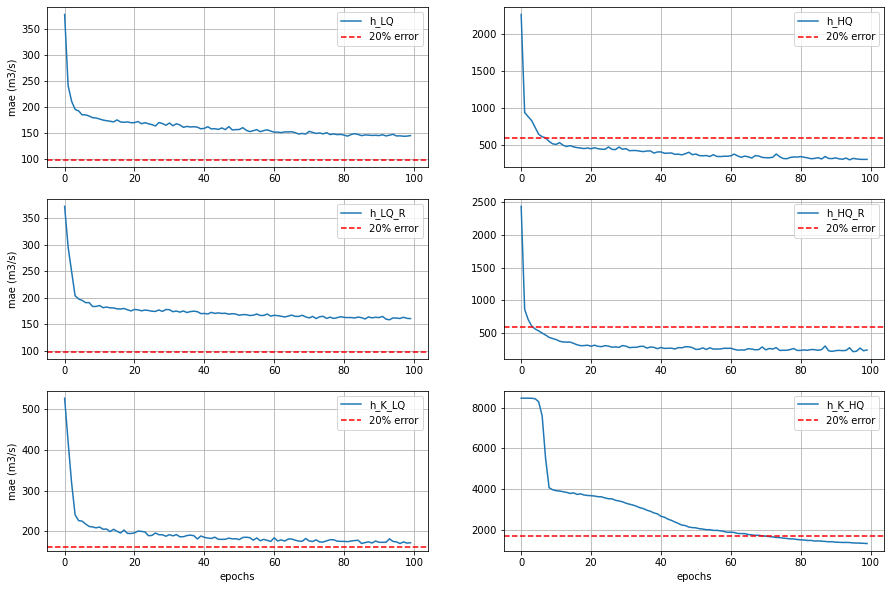
\includegraphics[scale = 0.45]{Graph/subplot_mae_h.png}
    \caption{Goodness of fit of the neural network for each HydroSwot class}
    \label{fig:subploth}
\end{figure}

We see that all the curves decrease suddenly during the first epochs, then much more slowly, and that they finally converge. We observe that the $MAE$ of the High Q classes always decreases below the 20\% error rate, while the $MAE$ of the Low Q classes does not.

Specifically, in the cases where the $20\%$ error limit is reached, the goodness of fit of the neural networks is very satisfying. However, having a goodness of fit as precise can lead to over fitting. We can explain this accuracy by the low number of data in each classes (see table \ref{Tab:class_prop}).

Concerning the curves which never reach the 20\% error limit, the goodness of fit of the neural networks is not as accurate as excepted. The fitting is difficult because of the high number of data and the variety of measurements in both classes.

Finally, the $MAE$ curve for the Hydroswot K-means - Low Q class decreases suddenly and stays just above the 20\% error rate, which is more accurate that the two other Low Q classes. In this case, the goodness of fit of the neural network is almost as precise as expected.

\begin{figure}[H]
    \centering
    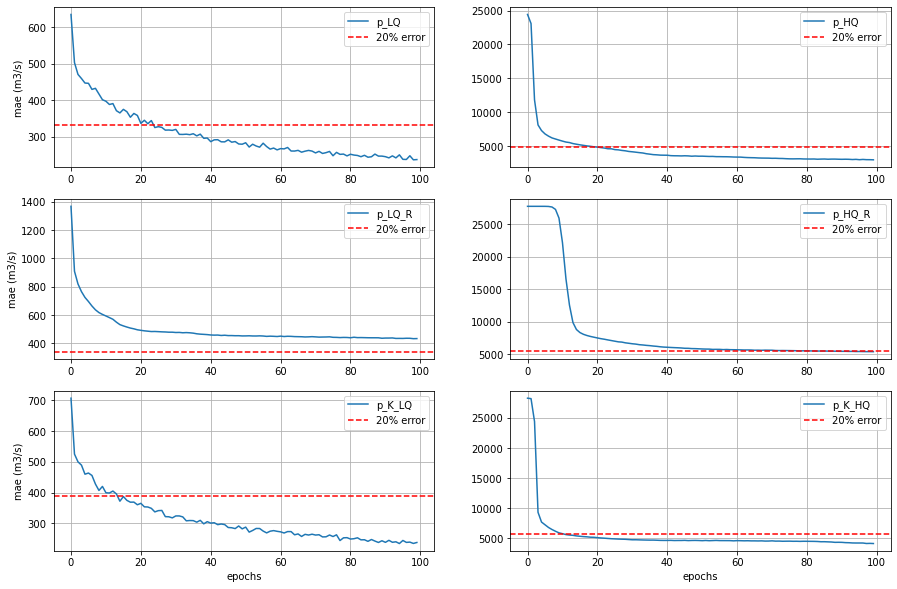
\includegraphics[scale = 0.45] {Graph/mae_subplot_pepsi.png}
    \caption{Goodness of fit of the neural network for each PEPSI class}
    \label{fig:mae pepsi}
\end{figure}

Figure \ref{fig:mae pepsi} shows the $MAE$ through the epochs for all the PEPSI classes. 
The $MAE$ behaviour for high Q classes is similar between them. The curves go closely under the 20\% of error rate. So, the goodness of fit is as expected. For the PEPSI handmade low Q full rivers class, the curve converges above the 20\% of error. Finally, the other low Q classes converge around 15\%. A hypothesis of this rate is the low number of rivers in these classes.   

\subsubsection{Artificial Neural Network testing.}

After the training of our neural networks, we evaluate their performances. Thus, we use the testing set - not used during the learning - to predict river discharge. First, we focus on the HydroSwot classes results. We verify the robustness of our neural networks with a Monte-Carlo method. Indeed, depending of the initialization of training and testing sets we obtain different results.  We initialize 20 times the training and testing sets, always with the same parameters. Then, we run the learning phase. We hence obtain results for 20 neural networks per classes. To quantify precisely the robustness of neural networks, we calculate the \textit{Normalized Root Mean Square Error} for all our classes. In Figure \ref{fig:MontecarloHydro}, we display the boxplots of the errors for all the HydroSwot classes.

\begin{figure}[H]
    \centering
    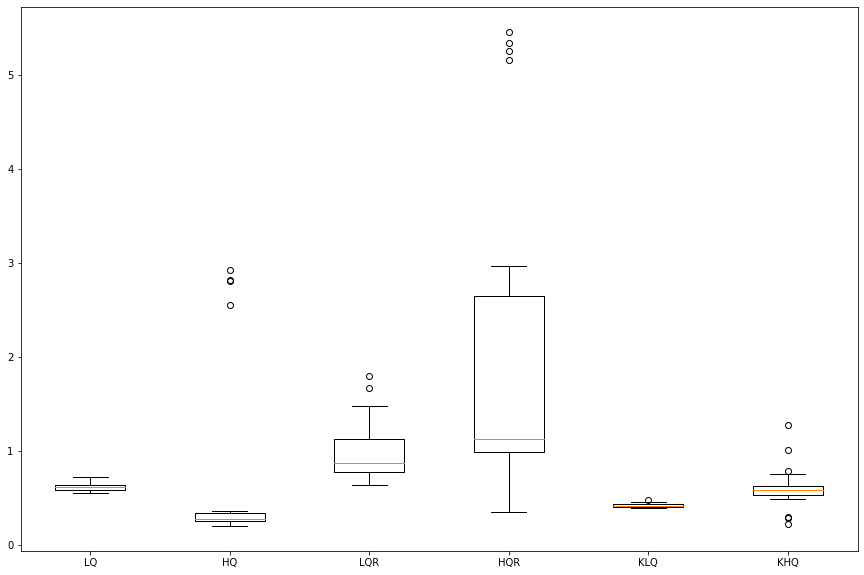
\includegraphics[scale = 0.3]{Graph/MonteCarlo_hydro.png}
    \caption{Boxplots of the \textit{nRMSE} errors for all HydroSwot classes}
    \label{fig:MontecarloHydro}
\end{figure}

 We clearly observe that the classes where we have full rivers contain much more errors, as the medians of the two boxplots are close to 1, and their ranges are much larger than the ones of other classes. Concerning the remaining boxplots, we show that the one with the best median is the HydroSwot Handmade - High Q, while the one with the smallest range is the HydroSwot K-means - Low Q. We also observe that high Q classes contains outliers, as opposed to the low Q classes, which are more robusts.

As a conclusion, classes which do not take full rivers present much better results. We also notice that the high Q classes can obtain the best predictions, but with a higher variance.


Now, we focus on PEPSI results. We plot the predictions (on the horizontal axis) against the real values (on the vertical axis). In figure \ref{fig:predictionsANN}, our predictions are computed on the PEPSI K-means classes.

\begin{figure}[H]
    \begin{subfigure}{0.45 \textwidth}
        \centering
        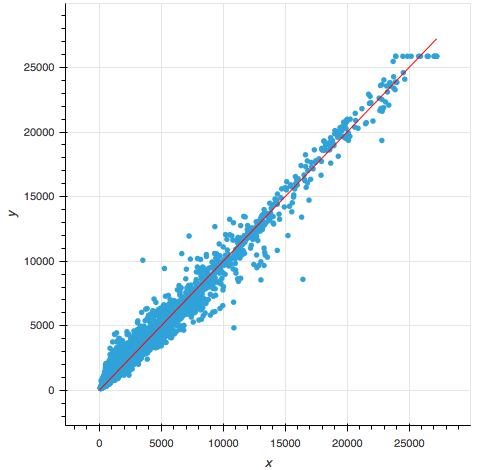
\includegraphics[scale = 0.4]{Graph/predictions_pepsiK_LQ.png}
        \caption{Low river discharge}
        \label{subfig:predLQ}
    \end{subfigure}
    \centering
     \begin{subfigure}{0.45 \textwidth}
         \centering
        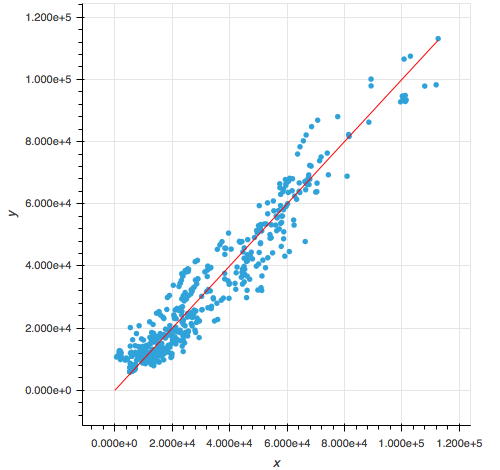
\includegraphics[scale = 0.4]{Graph/predictions_pepsiK_HQ.png}
        \caption{High river discharge}
        \label{subfig:predHQ}
     \end{subfigure}
 
 \caption{Predictions against real values of the neural network, PEPSI K-means - Low Q and High Q}
 \label{fig:predictionsANN}
\end{figure}

Figure \ref{subfig:predLQ} represents the predictions for low river discharges. We observe that the majority of the predictions are close to the red line, which means that a prediction is close to its real measure. We just observe some outliers, but their number is very small. In Figure \ref{subfig:predHQ}, we represent the predictions for high river discharges. Here, the predictions are further away from the red line. We assume this is due to the much smaller number of observations contained in this class compared to the low Q class. The predictions are good though.

Then, to focus on the predictions of a river in particular, we plot the predicted hydrographs of the rivers of the testing set, and we compare them to their true measures. Noteworthy that the hydrographs are only plotted when we use the classes with full rivers, since the other classes already use some observations of the rivers during training. The hydrographs can also be obtained only on the PEPSI dataset, because it is in this dataset that we have daily observations. Here, the following hydrographs (cf. Figure \ref{fig:hydrographKushiyara}, Figure \ref{fig:hydrographOhio}) come from the PEPSI Handmade Full rivers - Low Q class. 

\begin{figure}[H]
    \centering
    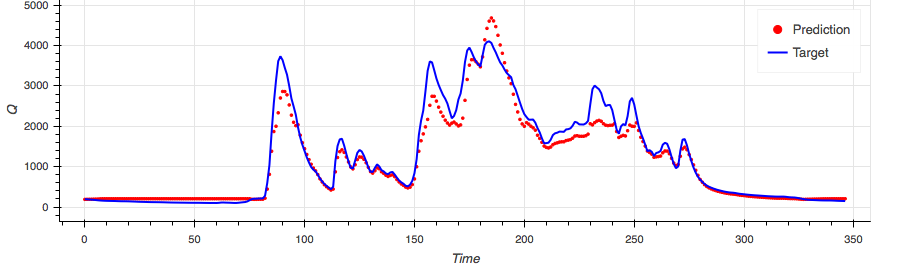
\includegraphics[scale = 0.4]{Graph/Hydrogramme_Kushiyara.png}
    \caption{Hydrograph of river $Kushiyara$, PEPSI low Q full river class}
    \label{fig:hydrographKushiyara}
\end{figure}
\begin{figure}[H]
    \centering
    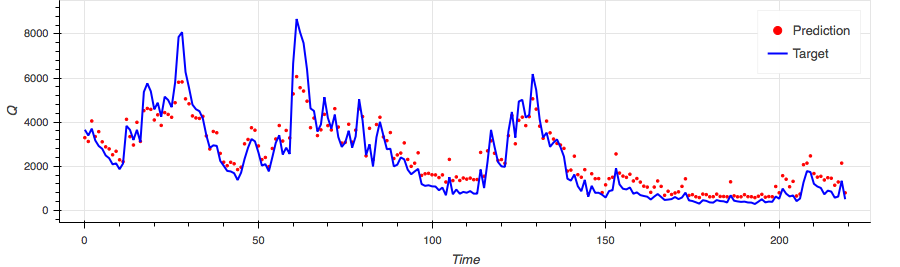
\includegraphics[scale = 0.4]{Graph/Hydrogramme_OhioSection2.png}
    \caption{Hydrograph of river Ohio - section 2, PEPSI low Q full river class}
    \label{fig:hydrographOhio}
\end{figure}

The accuracy of the predicted hydrographs vary depending on the river. We observe that the predicted hydrograph of river $Kushiyara$ fits well the real hydrograph: there is no temporal bias, all the peaks are present, and their values are close to reality (never more than a $800 m^3/s$ difference). However, the predicted hydrograph of river Ohio - Section 2 contains more bias while trying to predict the peaks, but there is again no temporal bias. 


\begin{table}[H]
    \centering
    \begin{tabular}{|c|c|}
    \hline
    Class & nRMSE \\ \hline \hline 
         p\_HQ& 0.19 \\ \hline
         p\_LQ& 0.32\\ \hline
         p\_HQ\_R & 2.46\\ \hline 
         p\_LQ\_R & 0.85\\ \hline
         p\_K\_HQ & 0.19\\ \hline
         p\_K\_LQ & 0.25\\ \hline
    \end{tabular}
    \caption{nRMSE calculated on testing sets for PEPSI classes}
    \label{tab:nRMSE-PEPSI}
\end{table}

Table \ref{tab:nRMSE-PEPSI} resumes neural networks performances for all PEPSI classes on testing set. The PEPSI Handmade Full rivers - High Q class does not have an accurate result. For this class, the training set is composed of 2 rivers and the testing set of only one river. Despite of the convergence of the $MAE$ to the 20\% of error rate (shown in figure \ref{fig:mae pepsi}), the neural network does not permit to estimate accurately the discharge of the third river. The PEPSI Handmade Full rivers - Low Q class does not have satisfying result. The reason can be the low number of river that the class have.


PEPSI Handmade - Low Q  and PEPSI K-means - Low Q classes have a $MAE$ on training set which decreased lower than the PEPSI Handmade - High Q and PEPSI K-means - High Q. However, their $nRMSE$ on testing set are worse than the other 2 classes. Hence, this result illustrates the phenomenon of over-fitting. 

We conclude of a good estimation of the discharge for all the PEPSI classes except for the full rivers ones.   